% Created by tikzDevice version 0.12.6 on 2024-12-17 18:06:00
% !TEX encoding = UTF-8 Unicode
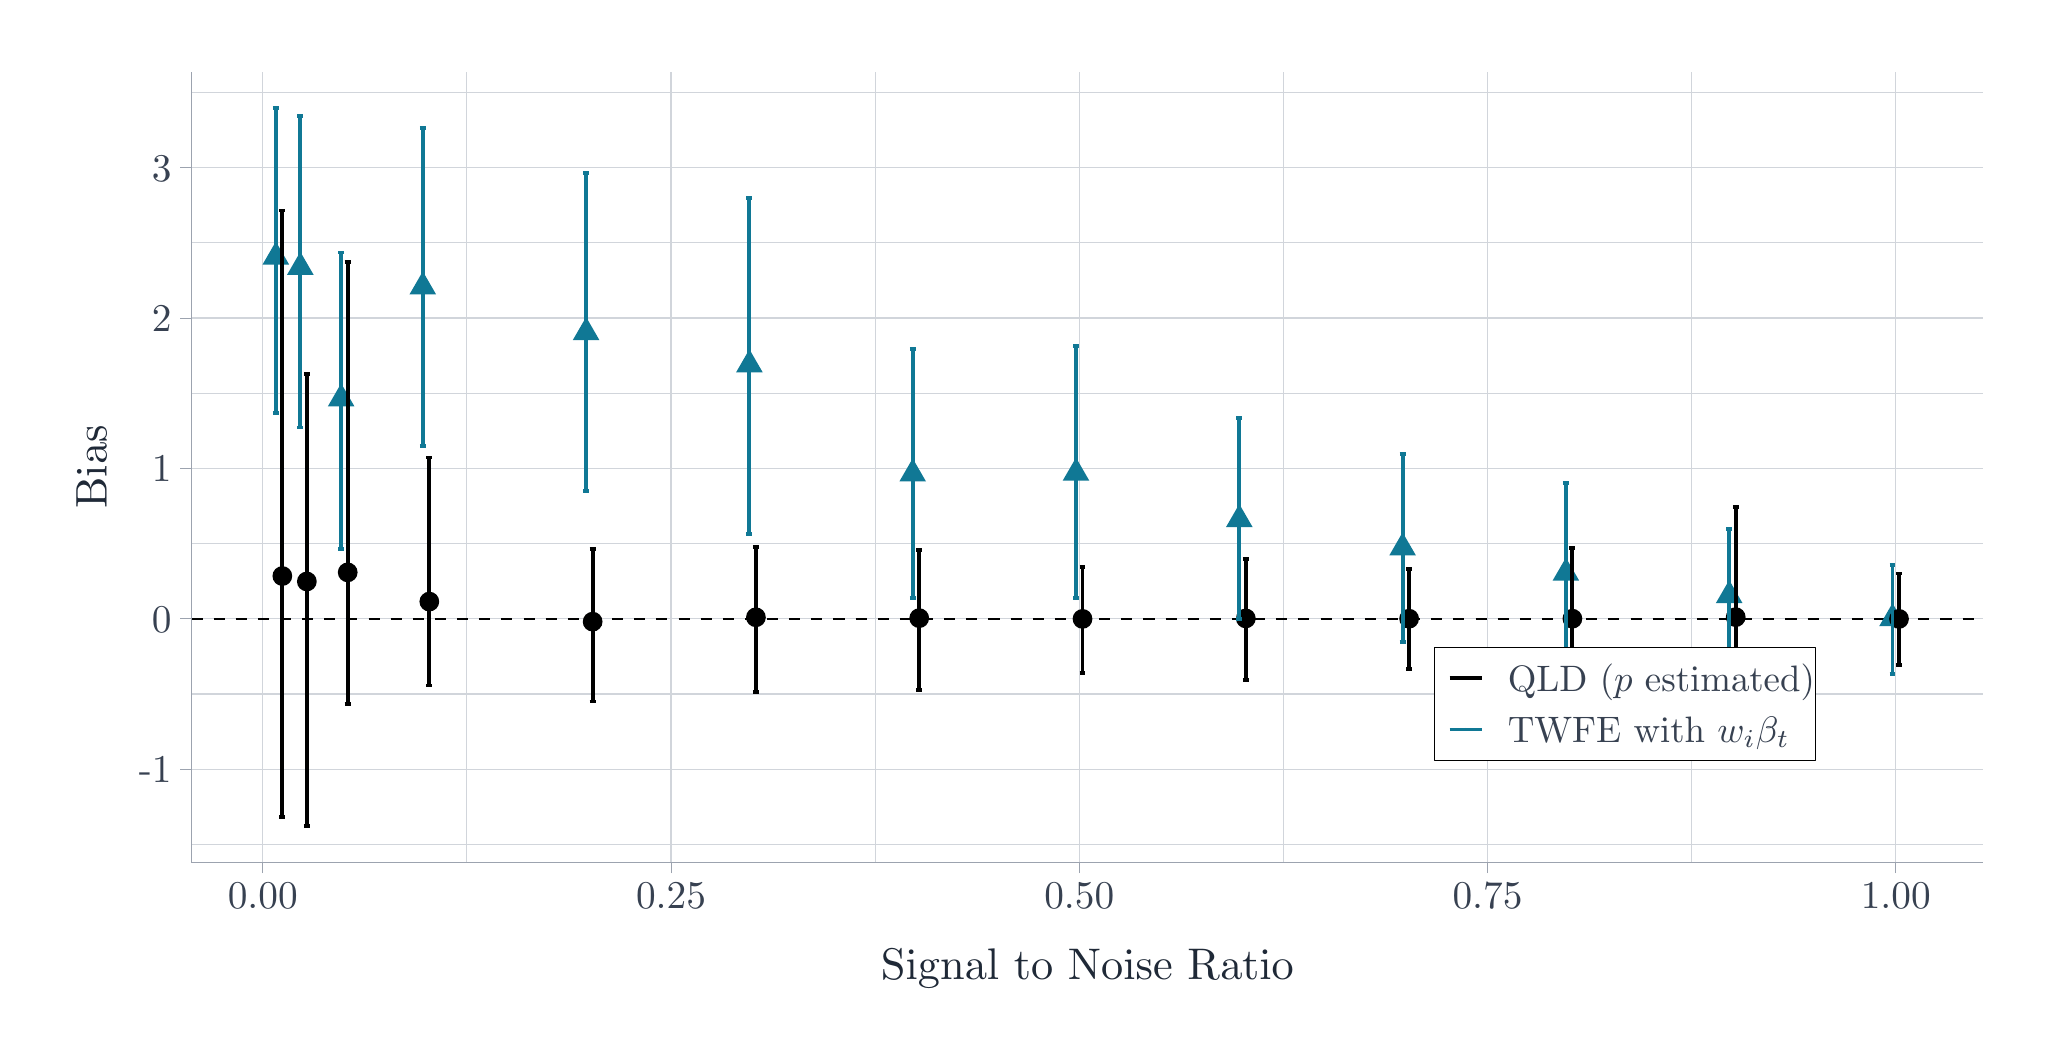
\begin{tikzpicture}[x=1pt,y=1pt]
\definecolor{fillColor}{RGB}{255,255,255}
\path[use as bounding box,fill=fillColor] (0,0) rectangle (722.70,361.35);
\begin{scope}
\path[clip] (  0.00,  0.00) rectangle (722.70,361.35);
\definecolor{drawColor}{RGB}{255,255,255}

\path[draw=drawColor,line width= 0.8pt,line join=round,line cap=round,fill=fillColor] (  0.00,  0.00) rectangle (722.70,361.35);
\end{scope}
\begin{scope}
\path[clip] ( 59.18, 59.89) rectangle (706.70,345.35);
\definecolor{drawColor}{RGB}{255,255,255}
\definecolor{fillColor}{RGB}{255,255,255}

\path[draw=drawColor,line width= 0.8pt,line join=round,line cap=round,fill=fillColor] ( 59.18, 59.89) rectangle (706.70,345.35);
\definecolor{drawColor}{RGB}{209,213,219}

\path[draw=drawColor,line width= 0.4pt,line join=round] ( 59.18, 66.20) --
	(706.70, 66.20);

\path[draw=drawColor,line width= 0.4pt,line join=round] ( 59.18,120.56) --
	(706.70,120.56);

\path[draw=drawColor,line width= 0.4pt,line join=round] ( 59.18,174.91) --
	(706.70,174.91);

\path[draw=drawColor,line width= 0.4pt,line join=round] ( 59.18,229.27) --
	(706.70,229.27);

\path[draw=drawColor,line width= 0.4pt,line join=round] ( 59.18,283.62) --
	(706.70,283.62);

\path[draw=drawColor,line width= 0.4pt,line join=round] ( 59.18,337.97) --
	(706.70,337.97);

\path[draw=drawColor,line width= 0.4pt,line join=round] (158.71, 59.89) --
	(158.71,345.35);

\path[draw=drawColor,line width= 0.4pt,line join=round] (306.23, 59.89) --
	(306.23,345.35);

\path[draw=drawColor,line width= 0.4pt,line join=round] (453.75, 59.89) --
	(453.75,345.35);

\path[draw=drawColor,line width= 0.4pt,line join=round] (601.27, 59.89) --
	(601.27,345.35);

\path[draw=drawColor,line width= 0.4pt,line join=round] ( 59.18, 93.38) --
	(706.70, 93.38);

\path[draw=drawColor,line width= 0.4pt,line join=round] ( 59.18,147.73) --
	(706.70,147.73);

\path[draw=drawColor,line width= 0.4pt,line join=round] ( 59.18,202.09) --
	(706.70,202.09);

\path[draw=drawColor,line width= 0.4pt,line join=round] ( 59.18,256.44) --
	(706.70,256.44);

\path[draw=drawColor,line width= 0.4pt,line join=round] ( 59.18,310.80) --
	(706.70,310.80);

\path[draw=drawColor,line width= 0.4pt,line join=round] ( 84.95, 59.89) --
	( 84.95,345.35);

\path[draw=drawColor,line width= 0.4pt,line join=round] (232.47, 59.89) --
	(232.47,345.35);

\path[draw=drawColor,line width= 0.4pt,line join=round] (379.99, 59.89) --
	(379.99,345.35);

\path[draw=drawColor,line width= 0.4pt,line join=round] (527.51, 59.89) --
	(527.51,345.35);

\path[draw=drawColor,line width= 0.4pt,line join=round] (675.02, 59.89) --
	(675.02,345.35);
\definecolor{drawColor}{RGB}{0,0,0}

\path[draw=drawColor,line width= 0.6pt,dash pattern=on 4pt off 4pt ,line join=round] ( 59.18,147.73) -- (706.70,147.73);
\definecolor{fillColor}{RGB}{16,120,149}

\path[fill=fillColor] ( 89.67,284.07) --
	( 94.48,275.75) --
	( 84.87,275.75) --
	cycle;
\definecolor{fillColor}{RGB}{0,0,0}

\path[fill=fillColor] ( 92.03,163.20) circle (  3.57);
\definecolor{fillColor}{RGB}{16,120,149}

\path[fill=fillColor] ( 98.52,280.36) --
	(103.33,272.03) --
	( 93.72,272.03) --
	cycle;
\definecolor{fillColor}{RGB}{0,0,0}

\path[fill=fillColor] (100.88,161.23) circle (  3.57);
\definecolor{fillColor}{RGB}{16,120,149}

\path[fill=fillColor] (113.27,232.82) --
	(118.08,224.50) --
	(108.47,224.50) --
	cycle;
\definecolor{fillColor}{RGB}{0,0,0}

\path[fill=fillColor] (115.64,164.52) circle (  3.57);
\definecolor{fillColor}{RGB}{16,120,149}

\path[fill=fillColor] (142.78,273.29) --
	(147.58,264.96) --
	(137.97,264.96) --
	cycle;
\definecolor{fillColor}{RGB}{0,0,0}

\path[fill=fillColor] (145.14,153.96) circle (  3.57);
\definecolor{fillColor}{RGB}{16,120,149}

\path[fill=fillColor] (201.79,256.78) --
	(206.59,248.46) --
	(196.98,248.46) --
	cycle;
\definecolor{fillColor}{RGB}{0,0,0}

\path[fill=fillColor] (204.15,146.71) circle (  3.57);
\definecolor{fillColor}{RGB}{16,120,149}

\path[fill=fillColor] (260.79,245.14) --
	(265.60,236.81) --
	(255.99,236.81) --
	cycle;
\definecolor{fillColor}{RGB}{0,0,0}

\path[fill=fillColor] (263.15,148.29) circle (  3.57);
\definecolor{fillColor}{RGB}{16,120,149}

\path[fill=fillColor] (319.80,205.69) --
	(324.61,197.37) --
	(314.99,197.37) --
	cycle;
\definecolor{fillColor}{RGB}{0,0,0}

\path[fill=fillColor] (322.16,147.98) circle (  3.57);
\definecolor{fillColor}{RGB}{16,120,149}

\path[fill=fillColor] (378.81,205.98) --
	(383.61,197.66) --
	(374.00,197.66) --
	cycle;
\definecolor{fillColor}{RGB}{0,0,0}

\path[fill=fillColor] (381.17,147.71) circle (  3.57);
\definecolor{fillColor}{RGB}{16,120,149}

\path[fill=fillColor] (437.82,189.21) --
	(442.62,180.89) --
	(433.01,180.89) --
	cycle;
\definecolor{fillColor}{RGB}{0,0,0}

\path[fill=fillColor] (440.18,147.88) circle (  3.57);
\definecolor{fillColor}{RGB}{16,120,149}

\path[fill=fillColor] (496.82,178.98) --
	(501.63,170.66) --
	(492.02,170.66) --
	cycle;
\definecolor{fillColor}{RGB}{0,0,0}

\path[fill=fillColor] (499.18,147.78) circle (  3.57);
\definecolor{fillColor}{RGB}{16,120,149}

\path[fill=fillColor] (555.83,169.85) --
	(560.64,161.52) --
	(551.02,161.52) --
	cycle;
\definecolor{fillColor}{RGB}{0,0,0}

\path[fill=fillColor] (558.19,147.78) circle (  3.57);
\definecolor{fillColor}{RGB}{16,120,149}

\path[fill=fillColor] (614.84,161.75) --
	(619.64,153.43) --
	(610.03,153.43) --
	cycle;
\definecolor{fillColor}{RGB}{0,0,0}

\path[fill=fillColor] (617.20,148.34) circle (  3.57);
\definecolor{fillColor}{RGB}{16,120,149}

\path[fill=fillColor] (673.84,153.40) --
	(678.65,145.07) --
	(669.04,145.07) --
	cycle;
\definecolor{fillColor}{RGB}{0,0,0}

\path[fill=fillColor] (676.21,147.71) circle (  3.57);
\definecolor{drawColor}{RGB}{16,120,149}

\path[draw=drawColor,line width= 1.4pt,line join=round] ( 88.61,332.37) --
	( 90.73,332.37);

\path[draw=drawColor,line width= 1.4pt,line join=round] ( 89.67,332.37) --
	( 89.67,222.15);

\path[draw=drawColor,line width= 1.4pt,line join=round] ( 88.61,222.15) --
	( 90.73,222.15);
\definecolor{drawColor}{RGB}{0,0,0}

\path[draw=drawColor,line width= 1.4pt,line join=round] ( 90.97,295.29) --
	( 93.09,295.29);

\path[draw=drawColor,line width= 1.4pt,line join=round] ( 92.03,295.29) --
	( 92.03, 76.04);

\path[draw=drawColor,line width= 1.4pt,line join=round] ( 90.97, 76.04) --
	( 93.09, 76.04);
\definecolor{drawColor}{RGB}{16,120,149}

\path[draw=drawColor,line width= 1.4pt,line join=round] ( 97.46,329.44) --
	( 99.59,329.44);

\path[draw=drawColor,line width= 1.4pt,line join=round] ( 98.52,329.44) --
	( 98.52,216.86);

\path[draw=drawColor,line width= 1.4pt,line join=round] ( 97.46,216.86) --
	( 99.59,216.86);
\definecolor{drawColor}{RGB}{0,0,0}

\path[draw=drawColor,line width= 1.4pt,line join=round] ( 99.82,236.18) --
	(101.95,236.18);

\path[draw=drawColor,line width= 1.4pt,line join=round] (100.88,236.18) --
	(100.88, 72.86);

\path[draw=drawColor,line width= 1.4pt,line join=round] ( 99.82, 72.86) --
	(101.95, 72.86);
\definecolor{drawColor}{RGB}{16,120,149}

\path[draw=drawColor,line width= 1.4pt,line join=round] (112.21,280.09) --
	(114.34,280.09);

\path[draw=drawColor,line width= 1.4pt,line join=round] (113.27,280.09) --
	(113.27,172.85);

\path[draw=drawColor,line width= 1.4pt,line join=round] (112.21,172.85) --
	(114.34,172.85);
\definecolor{drawColor}{RGB}{0,0,0}

\path[draw=drawColor,line width= 1.4pt,line join=round] (114.57,276.54) --
	(116.70,276.54);

\path[draw=drawColor,line width= 1.4pt,line join=round] (115.64,276.54) --
	(115.64,116.92);

\path[draw=drawColor,line width= 1.4pt,line join=round] (114.57,116.92) --
	(116.70,116.92);
\definecolor{drawColor}{RGB}{16,120,149}

\path[draw=drawColor,line width= 1.4pt,line join=round] (141.72,324.96) --
	(143.84,324.96);

\path[draw=drawColor,line width= 1.4pt,line join=round] (142.78,324.96) --
	(142.78,210.07);

\path[draw=drawColor,line width= 1.4pt,line join=round] (141.72,210.07) --
	(143.84,210.07);
\definecolor{drawColor}{RGB}{0,0,0}

\path[draw=drawColor,line width= 1.4pt,line join=round] (144.08,206.04) --
	(146.20,206.04);

\path[draw=drawColor,line width= 1.4pt,line join=round] (145.14,206.04) --
	(145.14,123.63);

\path[draw=drawColor,line width= 1.4pt,line join=round] (144.08,123.63) --
	(146.20,123.63);
\definecolor{drawColor}{RGB}{16,120,149}

\path[draw=drawColor,line width= 1.4pt,line join=round] (200.72,308.70) --
	(202.85,308.70);

\path[draw=drawColor,line width= 1.4pt,line join=round] (201.79,308.70) --
	(201.79,193.91);

\path[draw=drawColor,line width= 1.4pt,line join=round] (200.72,193.91) --
	(202.85,193.91);
\definecolor{drawColor}{RGB}{0,0,0}

\path[draw=drawColor,line width= 1.4pt,line join=round] (203.08,172.88) --
	(205.21,172.88);

\path[draw=drawColor,line width= 1.4pt,line join=round] (204.15,172.88) --
	(204.15,117.84);

\path[draw=drawColor,line width= 1.4pt,line join=round] (203.08,117.84) --
	(205.21,117.84);
\definecolor{drawColor}{RGB}{16,120,149}

\path[draw=drawColor,line width= 1.4pt,line join=round] (259.73,299.84) --
	(261.86,299.84);

\path[draw=drawColor,line width= 1.4pt,line join=round] (260.79,299.84) --
	(260.79,178.34);

\path[draw=drawColor,line width= 1.4pt,line join=round] (259.73,178.34) --
	(261.86,178.34);
\definecolor{drawColor}{RGB}{0,0,0}

\path[draw=drawColor,line width= 1.4pt,line join=round] (262.09,173.63) --
	(264.22,173.63);

\path[draw=drawColor,line width= 1.4pt,line join=round] (263.15,173.63) --
	(263.15,121.15);

\path[draw=drawColor,line width= 1.4pt,line join=round] (262.09,121.15) --
	(264.22,121.15);
\definecolor{drawColor}{RGB}{16,120,149}

\path[draw=drawColor,line width= 1.4pt,line join=round] (318.74,245.13) --
	(320.86,245.13);

\path[draw=drawColor,line width= 1.4pt,line join=round] (319.80,245.13) --
	(319.80,155.16);

\path[draw=drawColor,line width= 1.4pt,line join=round] (318.74,155.16) --
	(320.86,155.16);
\definecolor{drawColor}{RGB}{0,0,0}

\path[draw=drawColor,line width= 1.4pt,line join=round] (321.10,172.52) --
	(323.22,172.52);

\path[draw=drawColor,line width= 1.4pt,line join=round] (322.16,172.52) --
	(322.16,122.01);

\path[draw=drawColor,line width= 1.4pt,line join=round] (321.10,122.01) --
	(323.22,122.01);
\definecolor{drawColor}{RGB}{16,120,149}

\path[draw=drawColor,line width= 1.4pt,line join=round] (377.75,246.19) --
	(379.87,246.19);

\path[draw=drawColor,line width= 1.4pt,line join=round] (378.81,246.19) --
	(378.81,155.35);

\path[draw=drawColor,line width= 1.4pt,line join=round] (377.75,155.35) --
	(379.87,155.35);
\definecolor{drawColor}{RGB}{0,0,0}

\path[draw=drawColor,line width= 1.4pt,line join=round] (380.11,166.56) --
	(382.23,166.56);

\path[draw=drawColor,line width= 1.4pt,line join=round] (381.17,166.56) --
	(381.17,128.28);

\path[draw=drawColor,line width= 1.4pt,line join=round] (380.11,128.28) --
	(382.23,128.28);
\definecolor{drawColor}{RGB}{16,120,149}

\path[draw=drawColor,line width= 1.4pt,line join=round] (436.75,220.40) --
	(438.88,220.40);

\path[draw=drawColor,line width= 1.4pt,line join=round] (437.82,220.40) --
	(437.82,147.77);

\path[draw=drawColor,line width= 1.4pt,line join=round] (436.75,147.77) --
	(438.88,147.77);
\definecolor{drawColor}{RGB}{0,0,0}

\path[draw=drawColor,line width= 1.4pt,line join=round] (439.11,169.43) --
	(441.24,169.43);

\path[draw=drawColor,line width= 1.4pt,line join=round] (440.18,169.43) --
	(440.18,125.62);

\path[draw=drawColor,line width= 1.4pt,line join=round] (439.11,125.62) --
	(441.24,125.62);
\definecolor{drawColor}{RGB}{16,120,149}

\path[draw=drawColor,line width= 1.4pt,line join=round] (495.76,207.29) --
	(497.88,207.29);

\path[draw=drawColor,line width= 1.4pt,line join=round] (496.82,207.29) --
	(496.82,139.28);

\path[draw=drawColor,line width= 1.4pt,line join=round] (495.76,139.28) --
	(497.88,139.28);
\definecolor{drawColor}{RGB}{0,0,0}

\path[draw=drawColor,line width= 1.4pt,line join=round] (498.12,165.80) --
	(500.25,165.80);

\path[draw=drawColor,line width= 1.4pt,line join=round] (499.18,165.80) --
	(499.18,129.49);

\path[draw=drawColor,line width= 1.4pt,line join=round] (498.12,129.49) --
	(500.25,129.49);
\definecolor{drawColor}{RGB}{16,120,149}

\path[draw=drawColor,line width= 1.4pt,line join=round] (554.77,196.71) --
	(556.89,196.71);

\path[draw=drawColor,line width= 1.4pt,line join=round] (555.83,196.71) --
	(555.83,133.15);

\path[draw=drawColor,line width= 1.4pt,line join=round] (554.77,133.15) --
	(556.89,133.15);
\definecolor{drawColor}{RGB}{0,0,0}

\path[draw=drawColor,line width= 1.4pt,line join=round] (557.13,173.34) --
	(559.25,173.34);

\path[draw=drawColor,line width= 1.4pt,line join=round] (558.19,173.34) --
	(558.19,122.55);

\path[draw=drawColor,line width= 1.4pt,line join=round] (557.13,122.55) --
	(559.25,122.55);
\definecolor{drawColor}{RGB}{16,120,149}

\path[draw=drawColor,line width= 1.4pt,line join=round] (613.78,180.16) --
	(615.90,180.16);

\path[draw=drawColor,line width= 1.4pt,line join=round] (614.84,180.16) --
	(614.84,131.92);

\path[draw=drawColor,line width= 1.4pt,line join=round] (613.78,131.92) --
	(615.90,131.92);
\definecolor{drawColor}{RGB}{0,0,0}

\path[draw=drawColor,line width= 1.4pt,line join=round] (616.14,188.12) --
	(618.26,188.12);

\path[draw=drawColor,line width= 1.4pt,line join=round] (617.20,188.12) --
	(617.20,105.28);

\path[draw=drawColor,line width= 1.4pt,line join=round] (616.14,105.28) --
	(618.26,105.28);
\definecolor{drawColor}{RGB}{16,120,149}

\path[draw=drawColor,line width= 1.4pt,line join=round] (672.78,167.06) --
	(674.91,167.06);

\path[draw=drawColor,line width= 1.4pt,line join=round] (673.84,167.06) --
	(673.84,127.81);

\path[draw=drawColor,line width= 1.4pt,line join=round] (672.78,127.81) --
	(674.91,127.81);
\definecolor{drawColor}{RGB}{0,0,0}

\path[draw=drawColor,line width= 1.4pt,line join=round] (675.14,164.12) --
	(677.27,164.12);

\path[draw=drawColor,line width= 1.4pt,line join=round] (676.21,164.12) --
	(676.21,131.04);

\path[draw=drawColor,line width= 1.4pt,line join=round] (675.14,131.04) --
	(677.27,131.04);
\end{scope}
\begin{scope}
\path[clip] (  0.00,  0.00) rectangle (722.70,361.35);
\definecolor{drawColor}{RGB}{156,163,175}

\path[draw=drawColor,line width= 0.3pt,line join=round] ( 59.18, 59.89) --
	( 59.18,345.35);
\end{scope}
\begin{scope}
\path[clip] (  0.00,  0.00) rectangle (722.70,361.35);
\definecolor{drawColor}{RGB}{55,65,81}

\node[text=drawColor,anchor=base east,inner sep=0pt, outer sep=0pt, scale=  1.42] at ( 51.98, 88.48) {-1};

\node[text=drawColor,anchor=base east,inner sep=0pt, outer sep=0pt, scale=  1.42] at ( 51.98,142.84) {0};

\node[text=drawColor,anchor=base east,inner sep=0pt, outer sep=0pt, scale=  1.42] at ( 51.98,197.19) {1};

\node[text=drawColor,anchor=base east,inner sep=0pt, outer sep=0pt, scale=  1.42] at ( 51.98,251.55) {2};

\node[text=drawColor,anchor=base east,inner sep=0pt, outer sep=0pt, scale=  1.42] at ( 51.98,305.90) {3};
\end{scope}
\begin{scope}
\path[clip] (  0.00,  0.00) rectangle (722.70,361.35);
\definecolor{drawColor}{RGB}{156,163,175}

\path[draw=drawColor,line width= 0.3pt,line join=round] ( 55.18, 93.38) --
	( 59.18, 93.38);

\path[draw=drawColor,line width= 0.3pt,line join=round] ( 55.18,147.73) --
	( 59.18,147.73);

\path[draw=drawColor,line width= 0.3pt,line join=round] ( 55.18,202.09) --
	( 59.18,202.09);

\path[draw=drawColor,line width= 0.3pt,line join=round] ( 55.18,256.44) --
	( 59.18,256.44);

\path[draw=drawColor,line width= 0.3pt,line join=round] ( 55.18,310.80) --
	( 59.18,310.80);
\end{scope}
\begin{scope}
\path[clip] (  0.00,  0.00) rectangle (722.70,361.35);
\definecolor{drawColor}{RGB}{156,163,175}

\path[draw=drawColor,line width= 0.3pt,line join=round] ( 59.18, 59.89) --
	(706.70, 59.89);
\end{scope}
\begin{scope}
\path[clip] (  0.00,  0.00) rectangle (722.70,361.35);
\definecolor{drawColor}{RGB}{156,163,175}

\path[draw=drawColor,line width= 0.3pt,line join=round] ( 84.95, 55.89) --
	( 84.95, 59.89);

\path[draw=drawColor,line width= 0.3pt,line join=round] (232.47, 55.89) --
	(232.47, 59.89);

\path[draw=drawColor,line width= 0.3pt,line join=round] (379.99, 55.89) --
	(379.99, 59.89);

\path[draw=drawColor,line width= 0.3pt,line join=round] (527.51, 55.89) --
	(527.51, 59.89);

\path[draw=drawColor,line width= 0.3pt,line join=round] (675.02, 55.89) --
	(675.02, 59.89);
\end{scope}
\begin{scope}
\path[clip] (  0.00,  0.00) rectangle (722.70,361.35);
\definecolor{drawColor}{RGB}{55,65,81}

\node[text=drawColor,anchor=base,inner sep=0pt, outer sep=0pt, scale=  1.42] at ( 84.95, 42.89) {0.00};

\node[text=drawColor,anchor=base,inner sep=0pt, outer sep=0pt, scale=  1.42] at (232.47, 42.89) {0.25};

\node[text=drawColor,anchor=base,inner sep=0pt, outer sep=0pt, scale=  1.42] at (379.99, 42.89) {0.50};

\node[text=drawColor,anchor=base,inner sep=0pt, outer sep=0pt, scale=  1.42] at (527.51, 42.89) {0.75};

\node[text=drawColor,anchor=base,inner sep=0pt, outer sep=0pt, scale=  1.42] at (675.02, 42.89) {1.00};
\end{scope}
\begin{scope}
\path[clip] (  0.00,  0.00) rectangle (722.70,361.35);
\definecolor{drawColor}{RGB}{31,41,55}

\node[text=drawColor,anchor=base,inner sep=0pt, outer sep=0pt, scale=  1.60] at (382.94, 17.56) {Signal to Noise Ratio};
\end{scope}
\begin{scope}
\path[clip] (  0.00,  0.00) rectangle (722.70,361.35);
\definecolor{drawColor}{RGB}{31,41,55}

\node[text=drawColor,rotate= 90.00,anchor=base,inner sep=0pt, outer sep=0pt, scale=  1.60] at ( 28.57,202.62) {Bias};
\end{scope}
\begin{scope}
\path[clip] (  0.00,  0.00) rectangle (722.70,361.35);
\definecolor{drawColor}{RGB}{0,0,0}
\definecolor{fillColor}{RGB}{255,255,255}

\path[draw=drawColor,line width= 0.6pt,line join=round,line cap=round,fill=fillColor] (508.38, 96.53) rectangle (646.01,137.43);
\end{scope}
\begin{scope}
\path[clip] (  0.00,  0.00) rectangle (722.70,361.35);
\definecolor{drawColor}{RGB}{255,255,255}
\definecolor{fillColor}{RGB}{255,255,255}

\path[draw=drawColor,line width= 0.8pt,line join=round,line cap=round,fill=fillColor] (512.38,118.98) rectangle (526.84,133.43);
\end{scope}
\begin{scope}
\path[clip] (  0.00,  0.00) rectangle (722.70,361.35);
\definecolor{fillColor}{RGB}{0,0,0}

\path[fill=fillColor] (519.61,126.21) circle (  0.36);
\end{scope}
\begin{scope}
\path[clip] (  0.00,  0.00) rectangle (722.70,361.35);
\definecolor{drawColor}{RGB}{0,0,0}

\path[draw=drawColor,line width= 1.4pt,line join=round] (513.83,126.21) -- (525.39,126.21);
\end{scope}
\begin{scope}
\path[clip] (  0.00,  0.00) rectangle (722.70,361.35);
\definecolor{drawColor}{RGB}{255,255,255}
\definecolor{fillColor}{RGB}{255,255,255}

\path[draw=drawColor,line width= 0.8pt,line join=round,line cap=round,fill=fillColor] (512.38,100.53) rectangle (526.84,114.98);
\end{scope}
\begin{scope}
\path[clip] (  0.00,  0.00) rectangle (722.70,361.35);
\definecolor{fillColor}{RGB}{16,120,149}

\path[fill=fillColor] (519.61,108.31) --
	(520.09,107.48) --
	(519.13,107.48) --
	cycle;
\end{scope}
\begin{scope}
\path[clip] (  0.00,  0.00) rectangle (722.70,361.35);
\definecolor{drawColor}{RGB}{16,120,149}

\path[draw=drawColor,line width= 1.4pt,line join=round] (513.83,107.75) -- (525.39,107.75);
\end{scope}
\begin{scope}
\path[clip] (  0.00,  0.00) rectangle (722.70,361.35);
\definecolor{drawColor}{RGB}{55,65,81}

\node[text=drawColor,anchor=base west,inner sep=0pt, outer sep=0pt, scale=  1.33] at (534.84,121.62) {QLD ($p$ estimated)};
\end{scope}
\begin{scope}
\path[clip] (  0.00,  0.00) rectangle (722.70,361.35);
\definecolor{drawColor}{RGB}{55,65,81}

\node[text=drawColor,anchor=base west,inner sep=0pt, outer sep=0pt, scale=  1.33] at (534.84,103.16) {TWFE with $\bm{w}_i \beta_t$};
\end{scope}
\end{tikzpicture}
